\section{Introduction}
Brain Computer Interface (BCI) is a technique that exploits brain activity to control external devices.
Brain activity is monitored by looking at the activation/deactivation of groups of neurons in particular areas of the brain.
This task can be fulfilled by measuring either the changes in its internal blood flow, using functional magnetic resonance imaging (fMRI), or its electromagnetic activity, using detectors sensitive to electrical (EEG) or magnetic (MEG) fields.
\subsection{Motor Imagery}
Motor imagery is a change in the sensorimotor rhythm (SMR) of the primary motor cortex that appears when the motor areas are activated (e.g. when a motor task is imagined).
This activation is typically characterized by a decrease in amplitude of the SMR signal.
This decrease is due to the random alignment of neuronal electric dipoles appearing when a certain area of the brain is activated.
By looking at the EEG signal in both the spatial and frequency domain, it is possible to discriminate the imagined movement of different parts of the body, information that can be used for BCI. \\
In this report, we will show an example of BCI using motor imagery.

\section{Data acquisition}
Electroencephalogram data are acquired using electrodes placed on the scalp at precise positions, as shown in Figure \ref{fig:electrodes}.
\begin{figure}[h!]
   \centering
   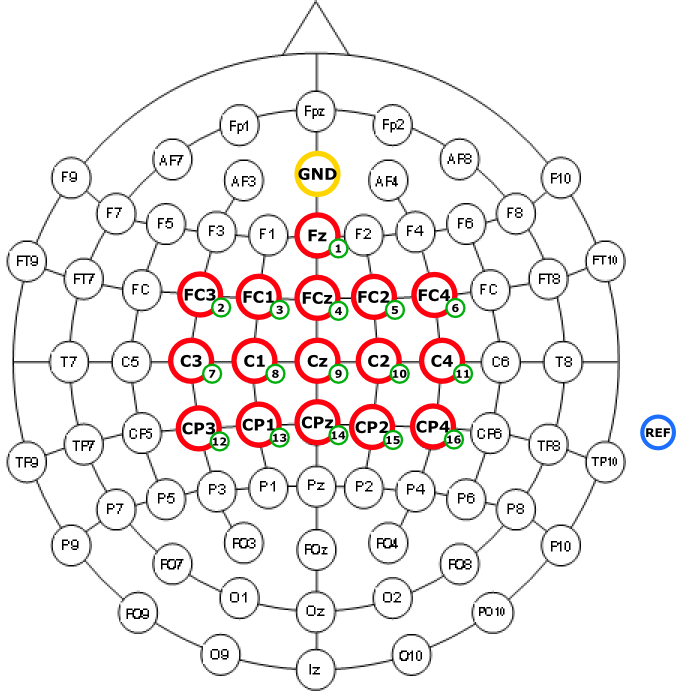
\includegraphics[width=0.8\textwidth]{images/electrodes.png}
   \caption{Spatial position of EEG electrodes. The electrodes used in the acquisition are marked in red and numbered from 1 to 16.}
   \label{fig:electrodes}
\end{figure}
Each electrode is identified by a name dependent on its position on the scalp and is associated with a number in our acquisition system.
EEG data are acquired at $\unit[512]{Hz}$ sample rate. \\
The acquisition is divided into two session, that will be referred to as ``offline'' and ``online'' session.
``Offline'' data are used to train the classifier, that is subsequently used to classify ``online'' data.
Both the ``offline'' and the ``online'' acquisition are divided into trials.
Each trial correspond to a single motor imagery.
The trials are divided into 3 classes, ``left hand'', ``right hand'' and ``both feet'', according to the movement the subject must imagine.
The ``offline'' session consists of 3 runs of 15 trials per class, giving a total of 135 trials.
The structure of a trial is shown in Figure \ref{fig:trial}.
\begin{figure}[h!]
   \centering
   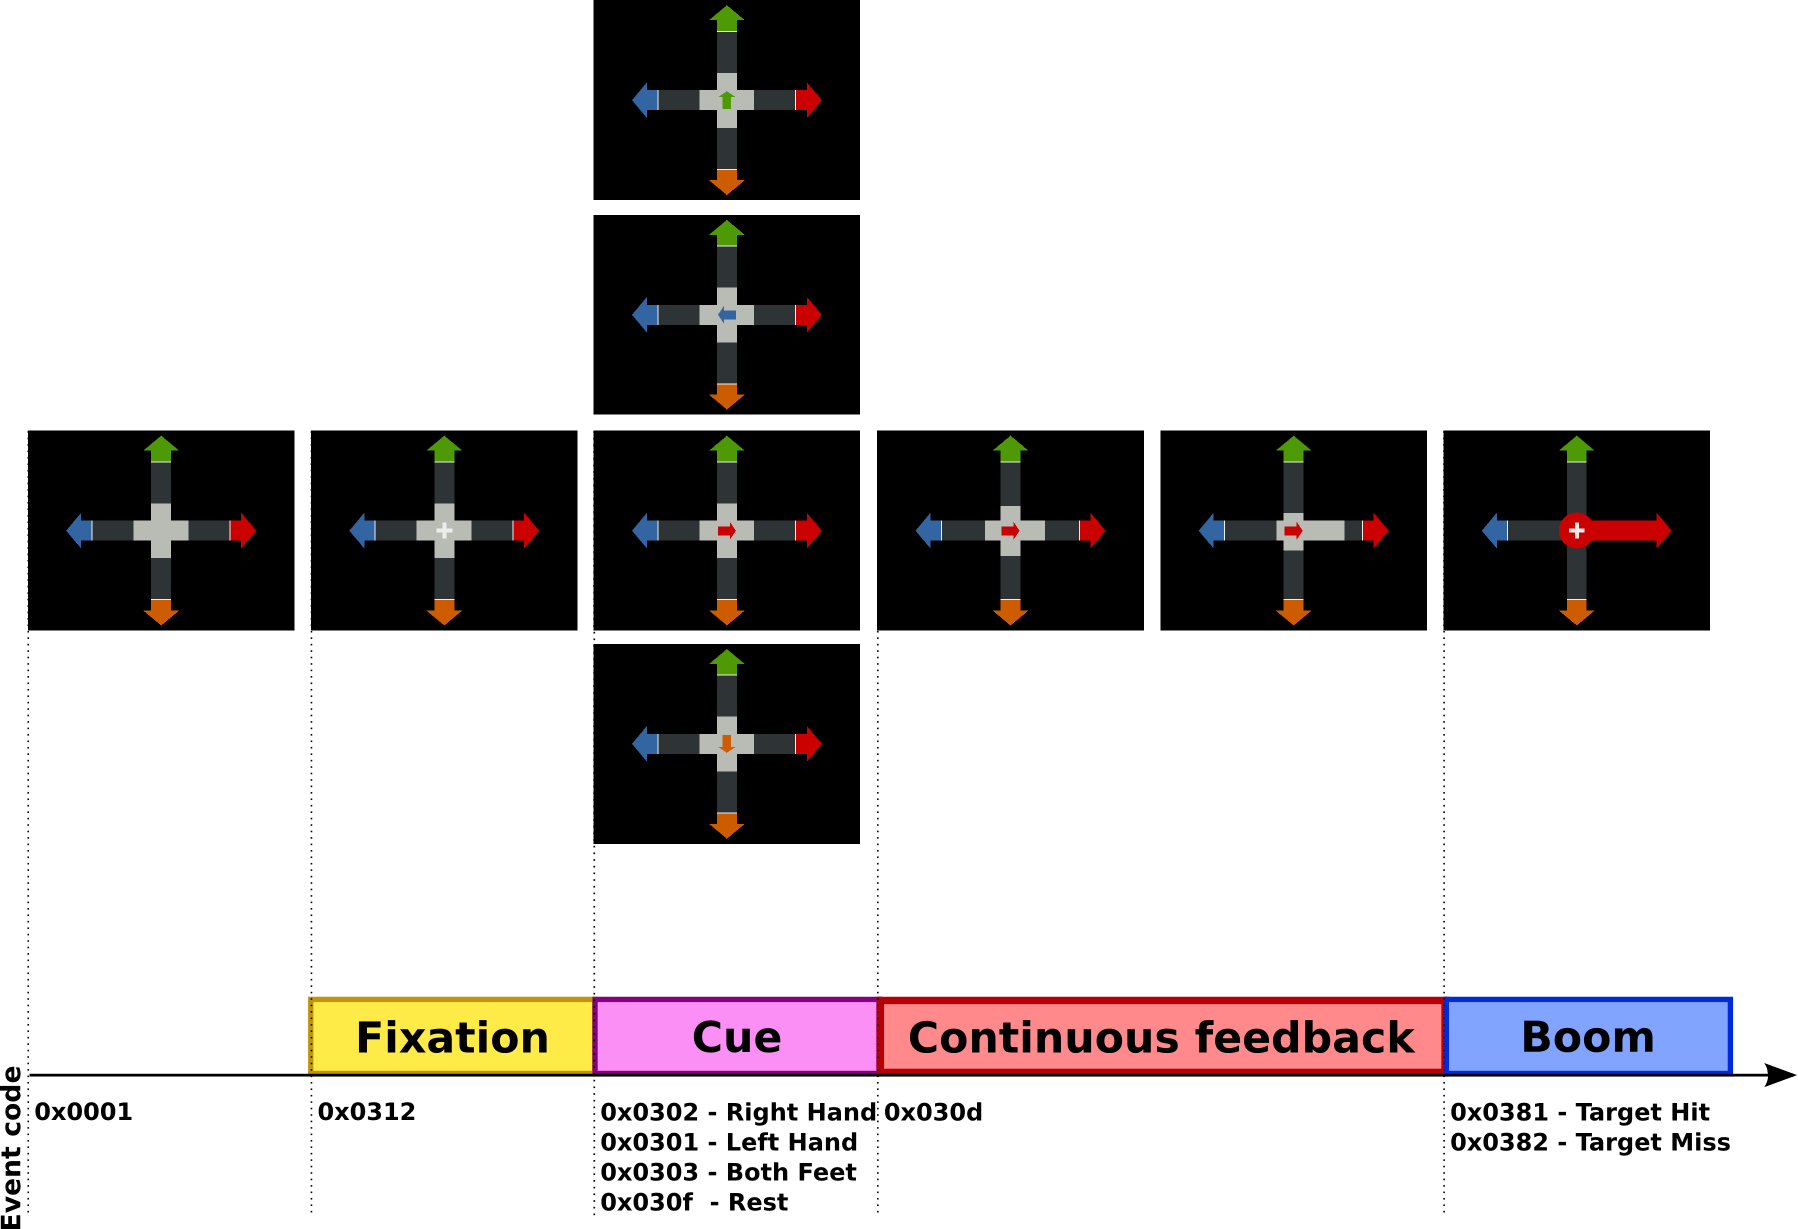
\includegraphics[width=\textwidth]{images/trial.png}
   \caption{Structure of a trial.}
   \label{fig:trial}
\end{figure}
At trial start, a 1 second fixation event is followed by the cue, where the subject is told the motor imagery he has to perform.
The cue is followed by 4 seconds of continuous feedback, where the subject is required to keep on imagining the movement, then the trial ends. \\
The ``online'' session, on the other hand, uses data from only two classes, ``left hand'' and ``both feet''.
It consists of 4 runs of 15 trials per class, for a total of 120 trials.
In the trials of this session, the classifier trained using ``offline'' data is used to discriminate between the two classes.
Therefore, during the continuous feedback, the probability of the recorded data to belong to each class is computed, until it reaches a certain threshold, after which the trial stops.
The end of the trial is marked with a ``hit'' event if the classifier has output the right class, with a ``miss'' event otherwise.

\section{Offline analysis}
The 3 runs of the ``offline'' session are divided into two sets: the first one (train set) is used to train the classifier while the second one (test set) is used to test it.
The train set is composed by the trials of the first 2 runs, while the last run is used as test set.

\subsection{Grand average results}
\subsubsection{EEG spectrum}
The EEG spectrum of the ``offline'' data is shown if Figures \ref{fig:EEG_RH}, \ref{fig:EEG_LH} and \ref{fig:EEG_BF} for, respectively, the ``right hand'', the ``left hand'' and the ``both feet'' class.
\begin{sidewaysfigure}[h!]
   \centering
   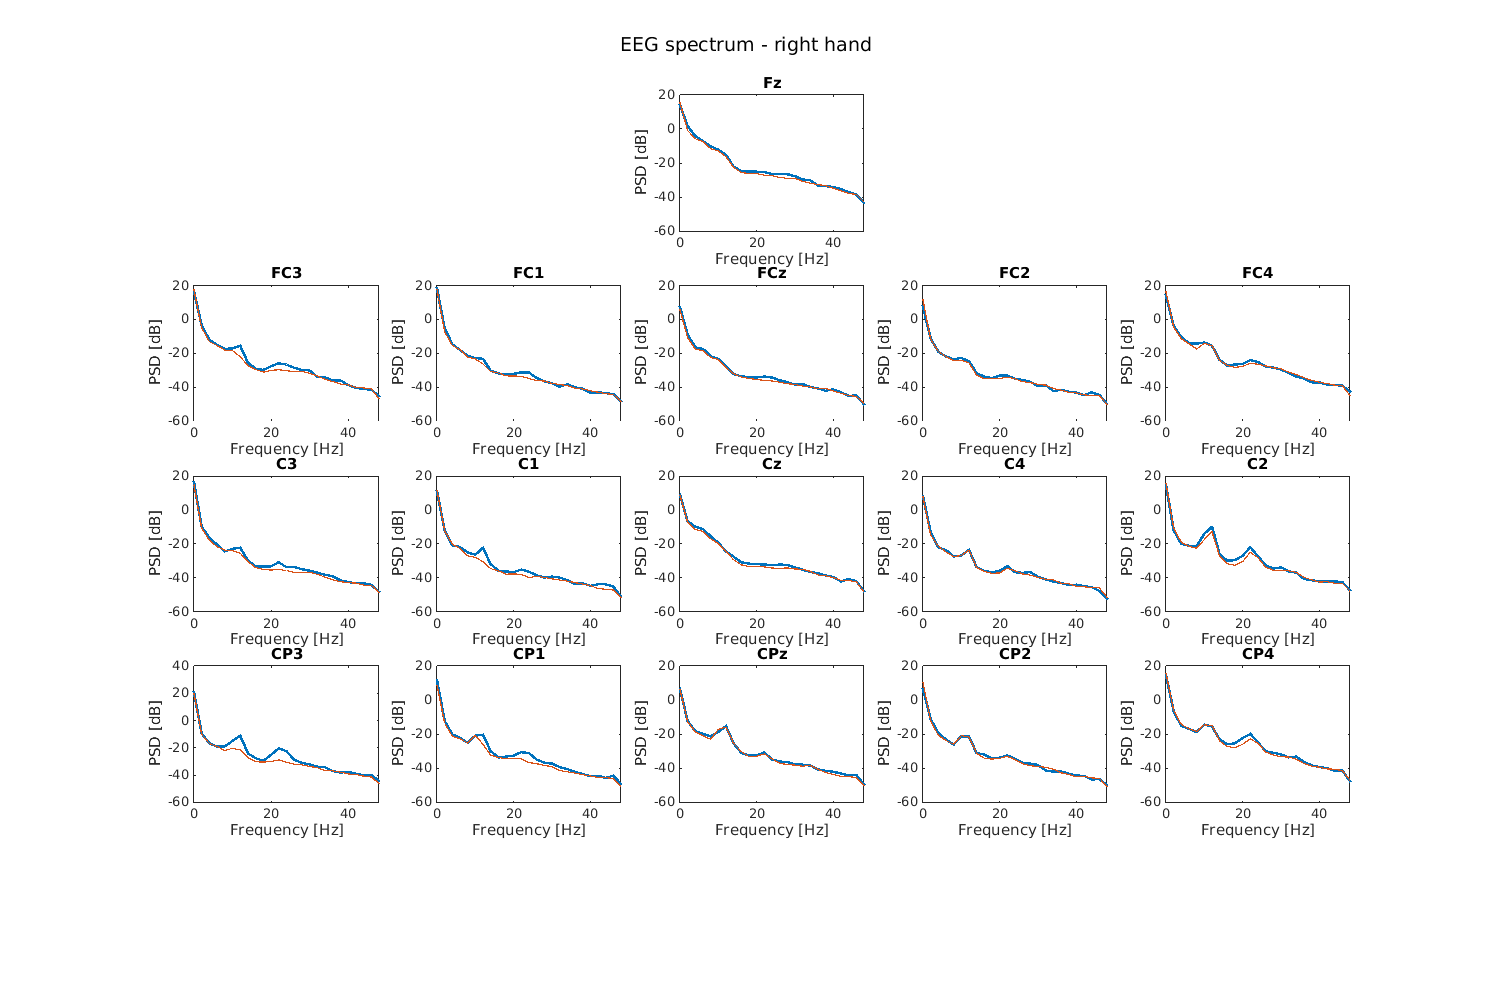
\includegraphics[width=\textwidth]{images/EEG_RH.png}
   \caption{EEG signal for the class ``right hand''. The blue, thick line corresponds to the baseline while the red, thin line to the task.}
   \label{fig:EEG_RH}
\end{sidewaysfigure}
\begin{sidewaysfigure}[h!]
   \centering
   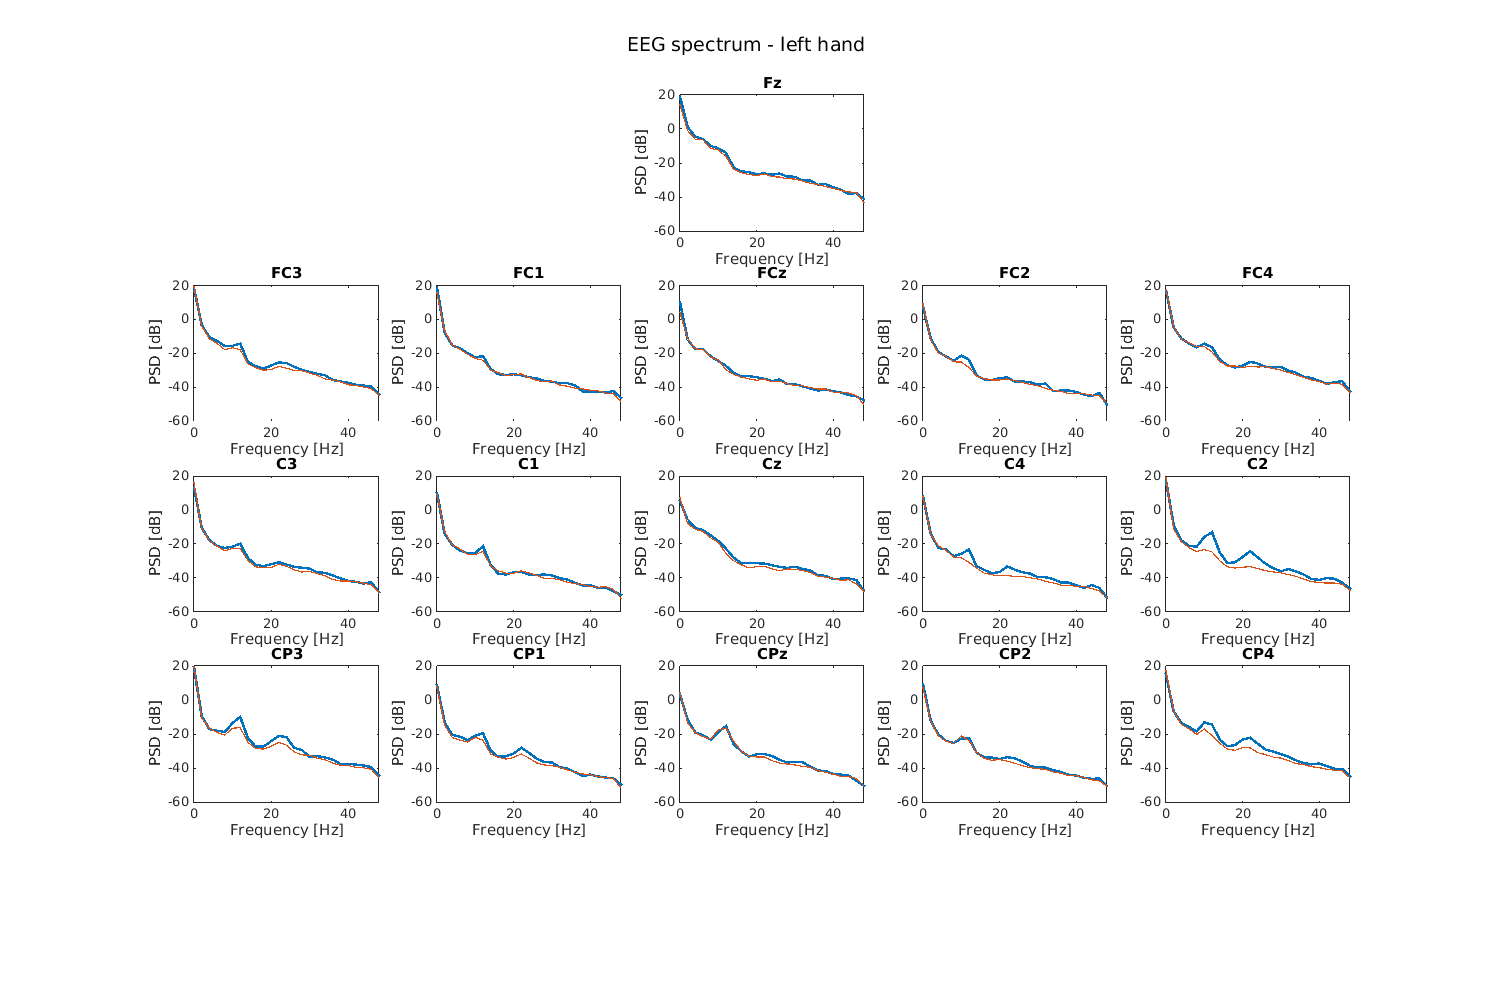
\includegraphics[width=\textwidth]{images/EEG_LH.png}
   \caption{EEG signal for the class ``left hand''. The blue, thick line corresponds to the baseline while the red, thin line to the task.}
   \label{fig:EEG_LH}
\end{sidewaysfigure}
\begin{sidewaysfigure}[h!]
   \centering
   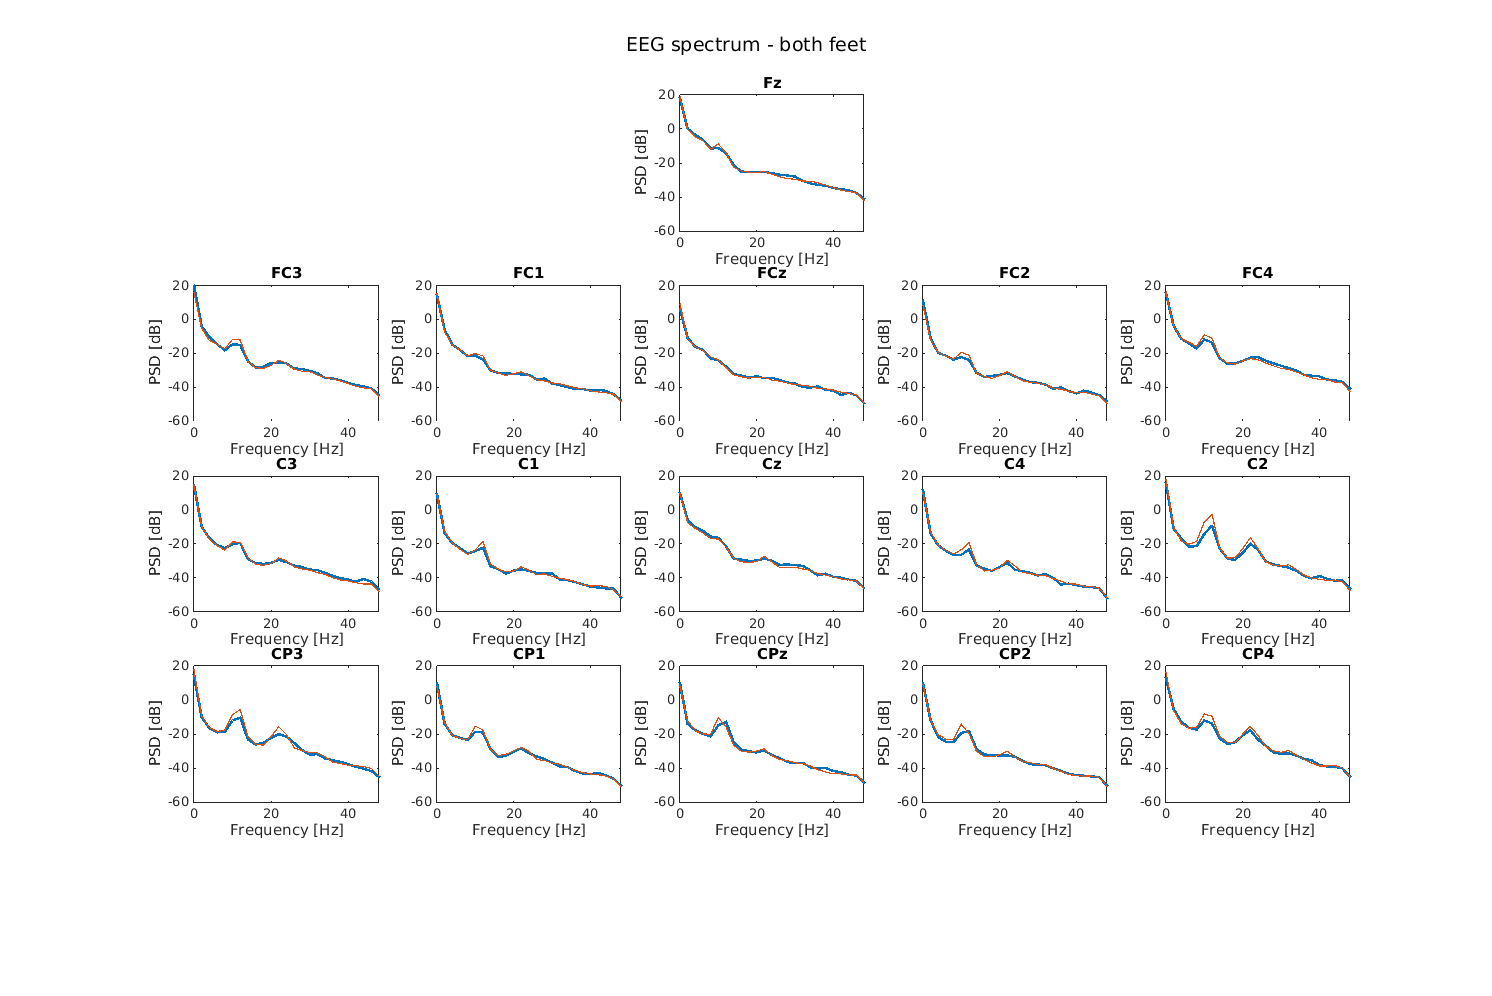
\includegraphics[width=\textwidth]{images/EEG_BF.png}
   \caption{EEG signal for the class ``both feet''. The blue, thick line corresponds to the baseline while the red, thin line to the task.}
   \label{fig:EEG_BF}
\end{sidewaysfigure}
The Figures compare the EEG spectrum of the baseline (between the start of the trial and the cue) and the task (from the cue to the end of the trial).
All the spectra show the typical $1/f$ trend.
The brain activity due to the task is evident for the classes ``right hand'' and ``left hand'' (see Figures \ref{fig:EEG_RH} and \ref{fig:EEG_LH}), with signal decrease of the electrodes respectively in the left hemisphere (Fig. \ref{fig:EEG_RH}) and in the right hemisphere (Fig. \ref{fig:EEG_LH}).
This decrease is the sign of a higher activity in those areas of the brain.

\subsubsection{ERD/ERS}
The temporal structure of this activity can be visualized by looking at the Event Related Desynchronization/Synchronization (ERD/ERS) as a function of time.
The ERD/ERS is the percentage change of the power spectral density (PSD) during the task related to the PSD of the baseline.
The ERD/ERS for the three classes is plot in the Figures \ref{fig:ERD_RH}, \ref{fig:ERD_LH} and \ref{fig:ERD_BF}.
\begin{sidewaysfigure}[h!]
   \centering
   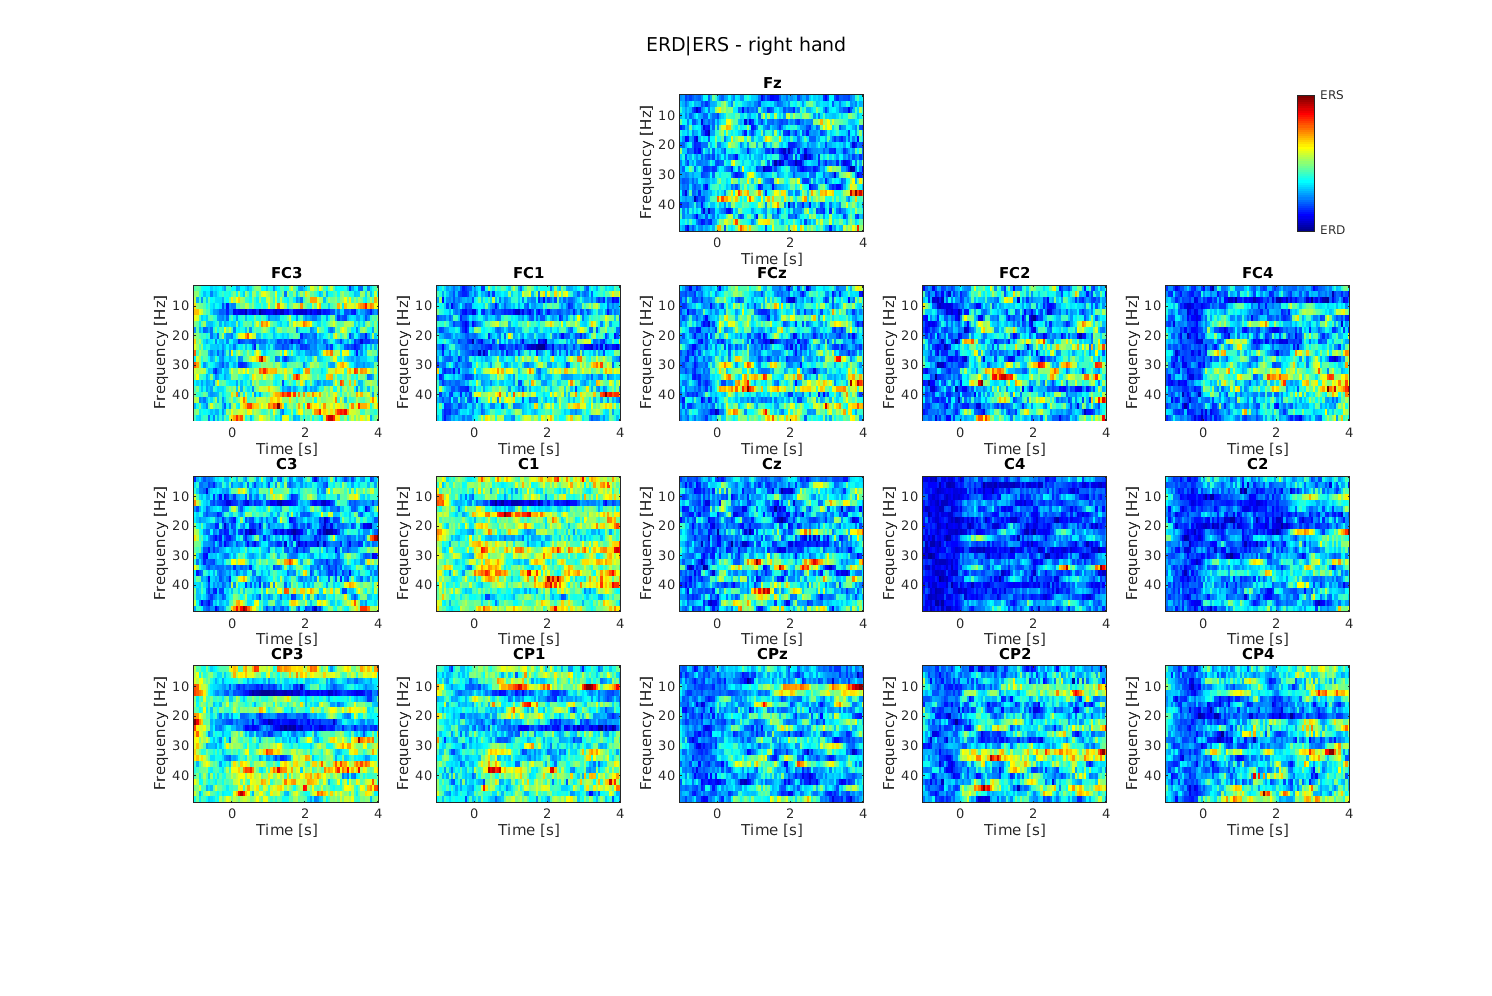
\includegraphics[width=\textwidth]{images/ERD_RH.png}
   \caption{ERD/ERS for the class ``right hand''. The cue is at $Time = 0$, with the baseline for negative times and the task for positive times.}
   \label{fig:ERD_RH}
\end{sidewaysfigure}
\begin{sidewaysfigure}[h!]
   \centering
   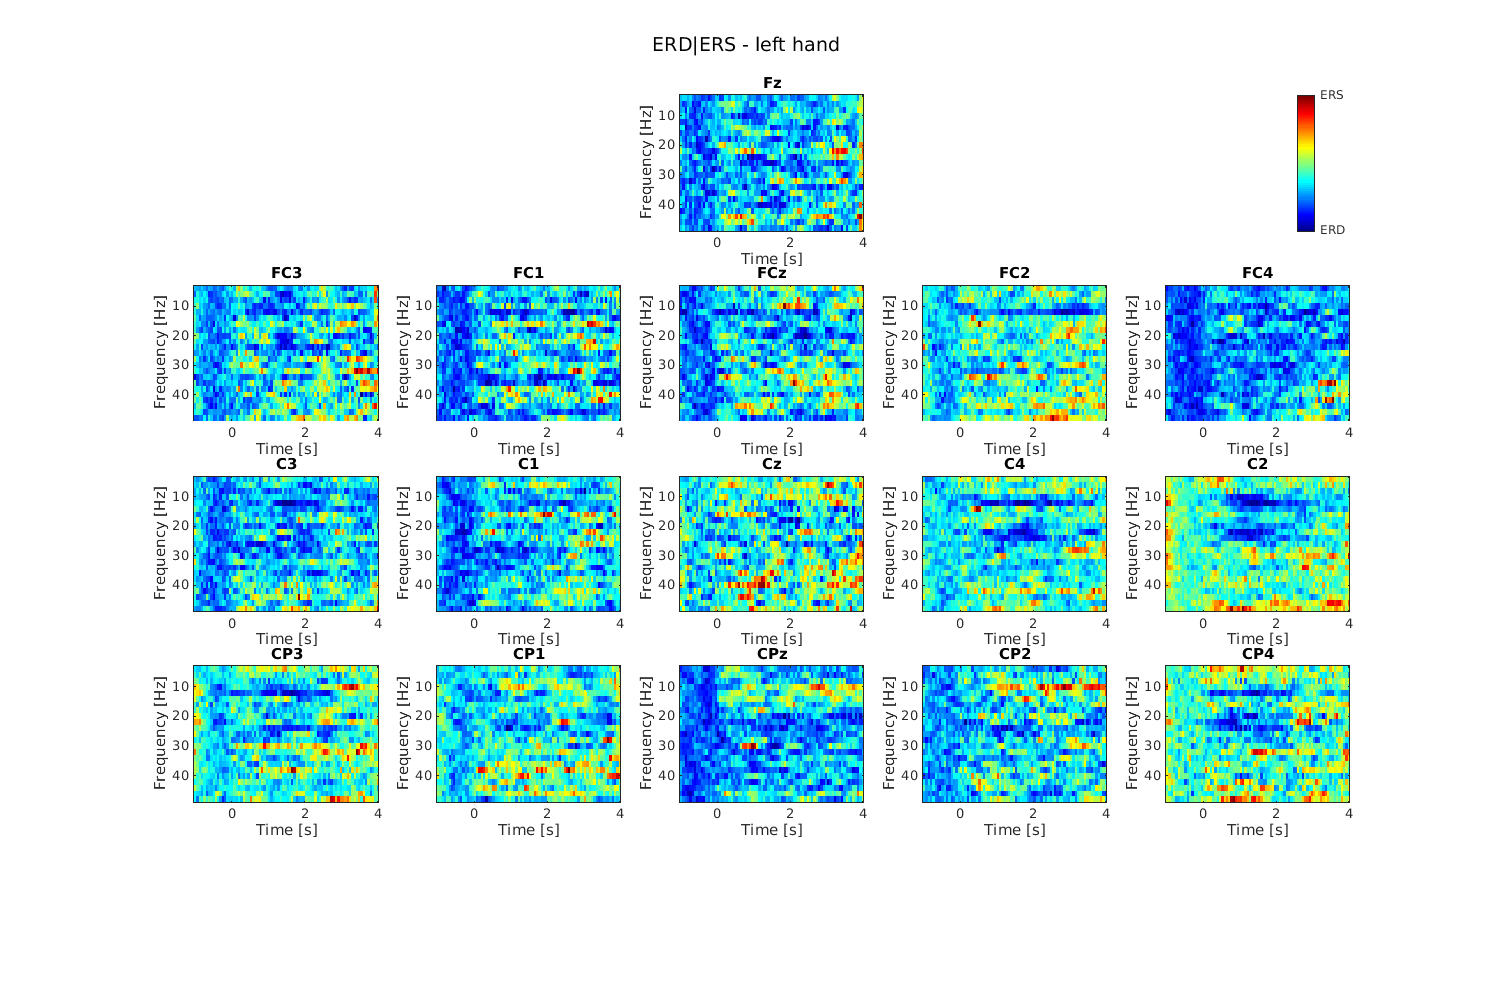
\includegraphics[width=\textwidth]{images/ERD_LH.png}
   \caption{ERD/ERS for the class ``left hand''. The cue is at $Time = 0$, with the baseline for negative times and the task for positive times.}
   \label{fig:ERD_LH}
\end{sidewaysfigure}
\begin{sidewaysfigure}[h!]
   \centering
   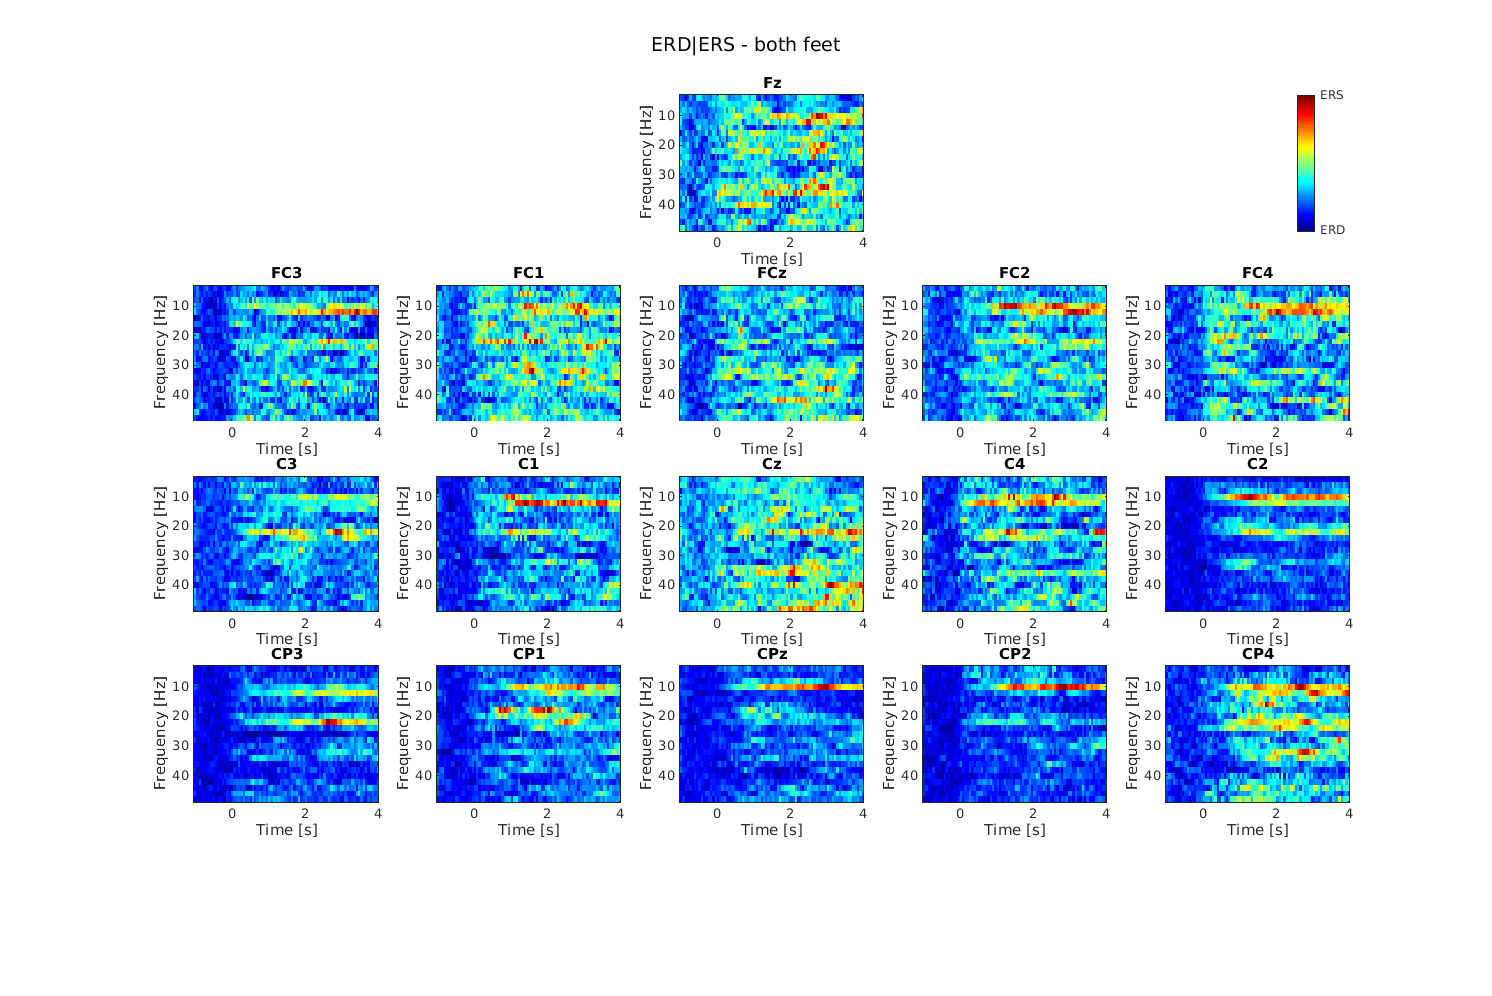
\includegraphics[width=\textwidth]{images/ERD_BF.png}
   \caption{ERD/ERS for the class ``both feet''. The cue is at $Time = 0$, with the baseline for negative times and the task for positive times.}
   \label{fig:ERD_BF}
\end{sidewaysfigure}
The decrease of the PSD already noticed in the EEG gives, for the classes right hand and left hand, the strong ERD that can be seen in Figures \ref{fig:ERD_RH} and \ref{fig:ERD_LH}, for frequencies between $10$ and $\unit[20]{Hz}$.
This effect starts at $Time = 0$ (the cue), therefore underlining its correlation with motor imagery.

\subsection{SMR classification}
All the steps of SMR classification are performed on the train data only.
In this way, it is possible to use the remaining data to test the accuracy of the classification.
\subsubsection{Feature selection}
The aim of SMR BCI is to tell for each instant which motor imagery the subject was performing.
This information can be extracted from the EEG by looking at its instantaneous power spectral density (PSD).
This quantity, however, is characterized by both frequency and channel, giving an enormous number of features that can be used for classification.
Such a large number is deleterious because it makes classification a very time consuming task, the contrary of what is expected from a system used to control an external device.
Moreover, since most features are not relevant for the classification, the only effect of their presence is to add noise, thus decreasing the efficacy of classification.
This is why it is necessary to select the features that are most significant for the desired classification. \\
In this report, we base feature selection upon Canonical Variates Analysis (CVA).
Given a set of data, belonging to two different classes, in a multidimensional space (in this case, with dimension equal to the number of features), CVA computes the discriminant power between the classes for each feature.
The results of CVA are shown in Figures \ref{fig:DP_LHRH}, \ref{fig:DP_RHBF} and \ref{fig:DP_LHBF} for, respectively, the couples of classes \{``left hand'', ``right hand''\}, \{``right hand'', ``both feet''\} and \{``left hand'', ``both feet''\}.
\begin{figure}[h!]
   \centering
   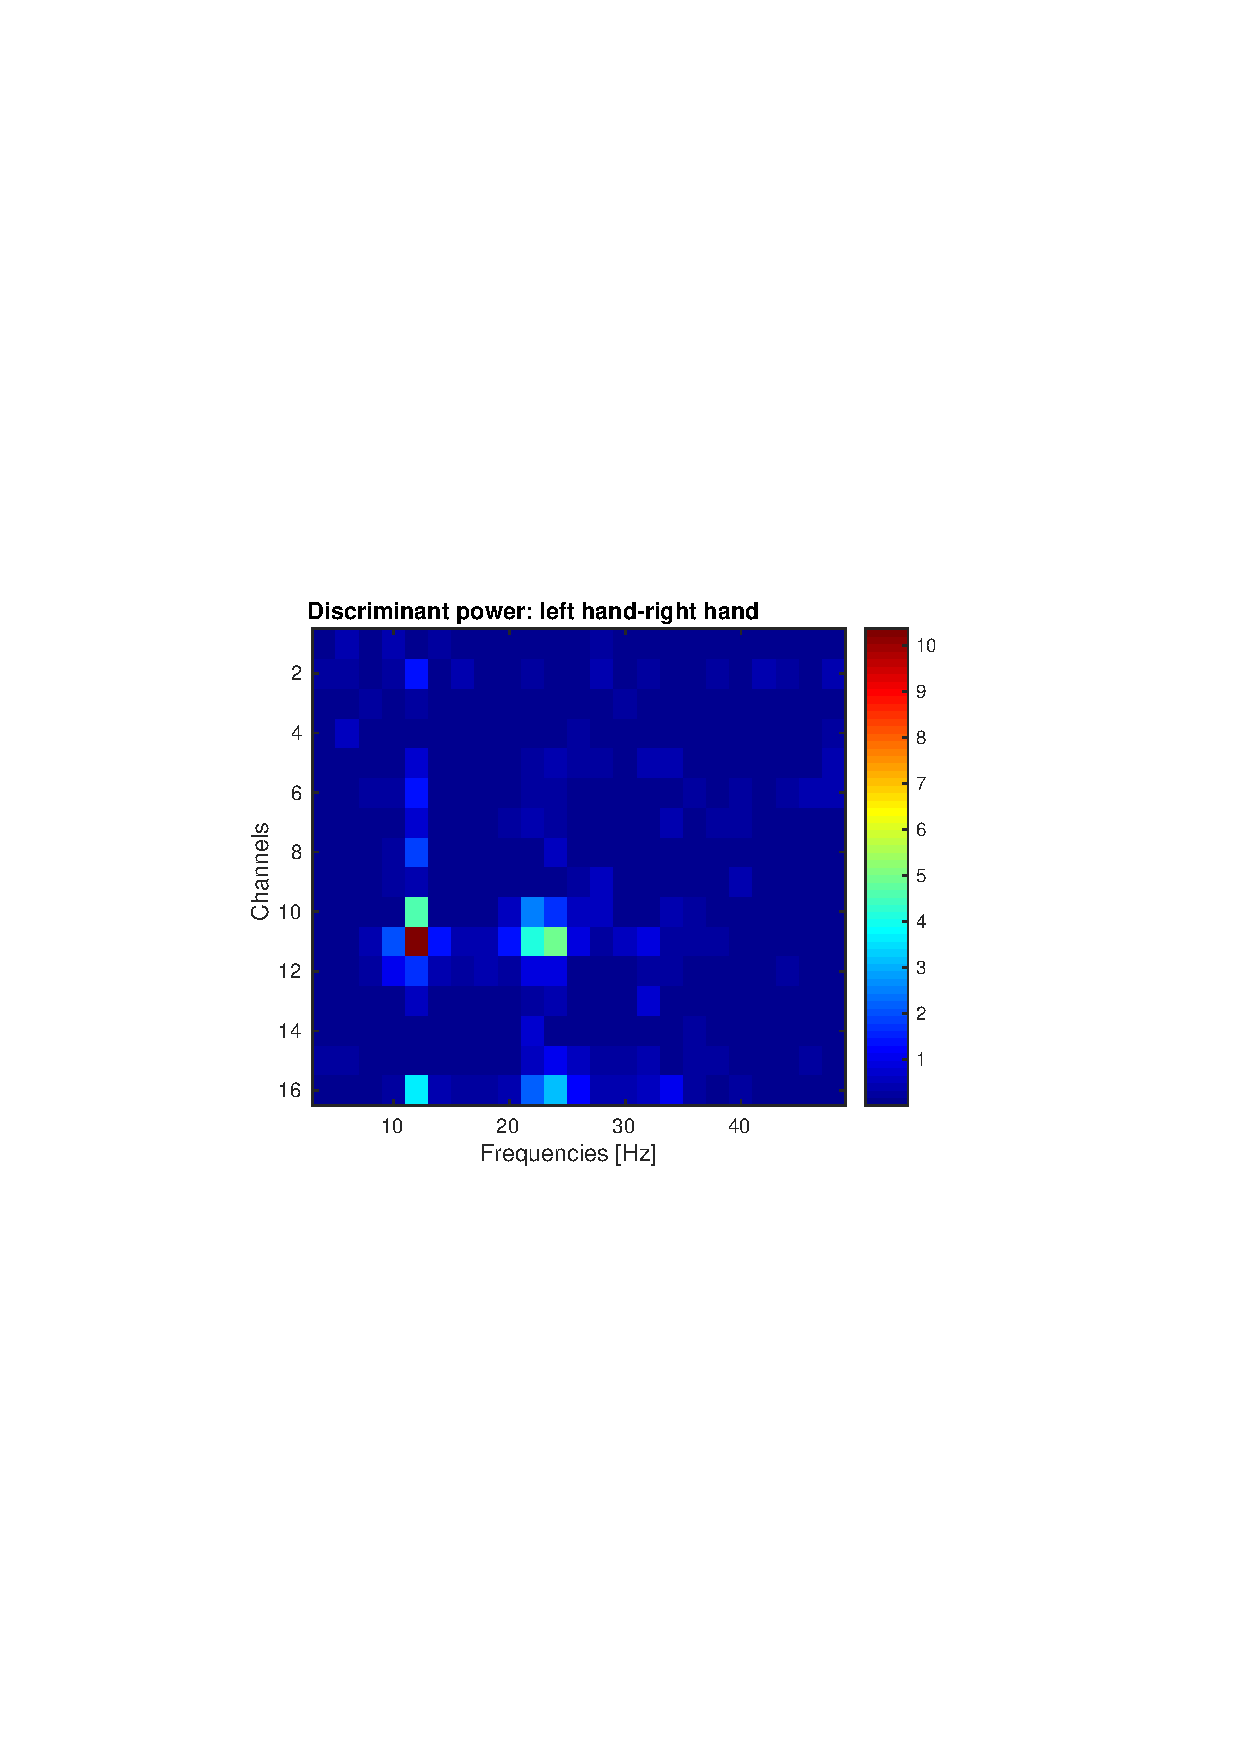
\includegraphics[width = \textwidth]{images/DP_LHRH.pdf}
   \caption{Discriminant power for the different features (channel,frequency) in the discrimination of the classes ``left hand'' and ``right hand''.}
   \label{fig:DP_LHRH}
\end{figure}
\begin{figure}[h!]
   \centering
   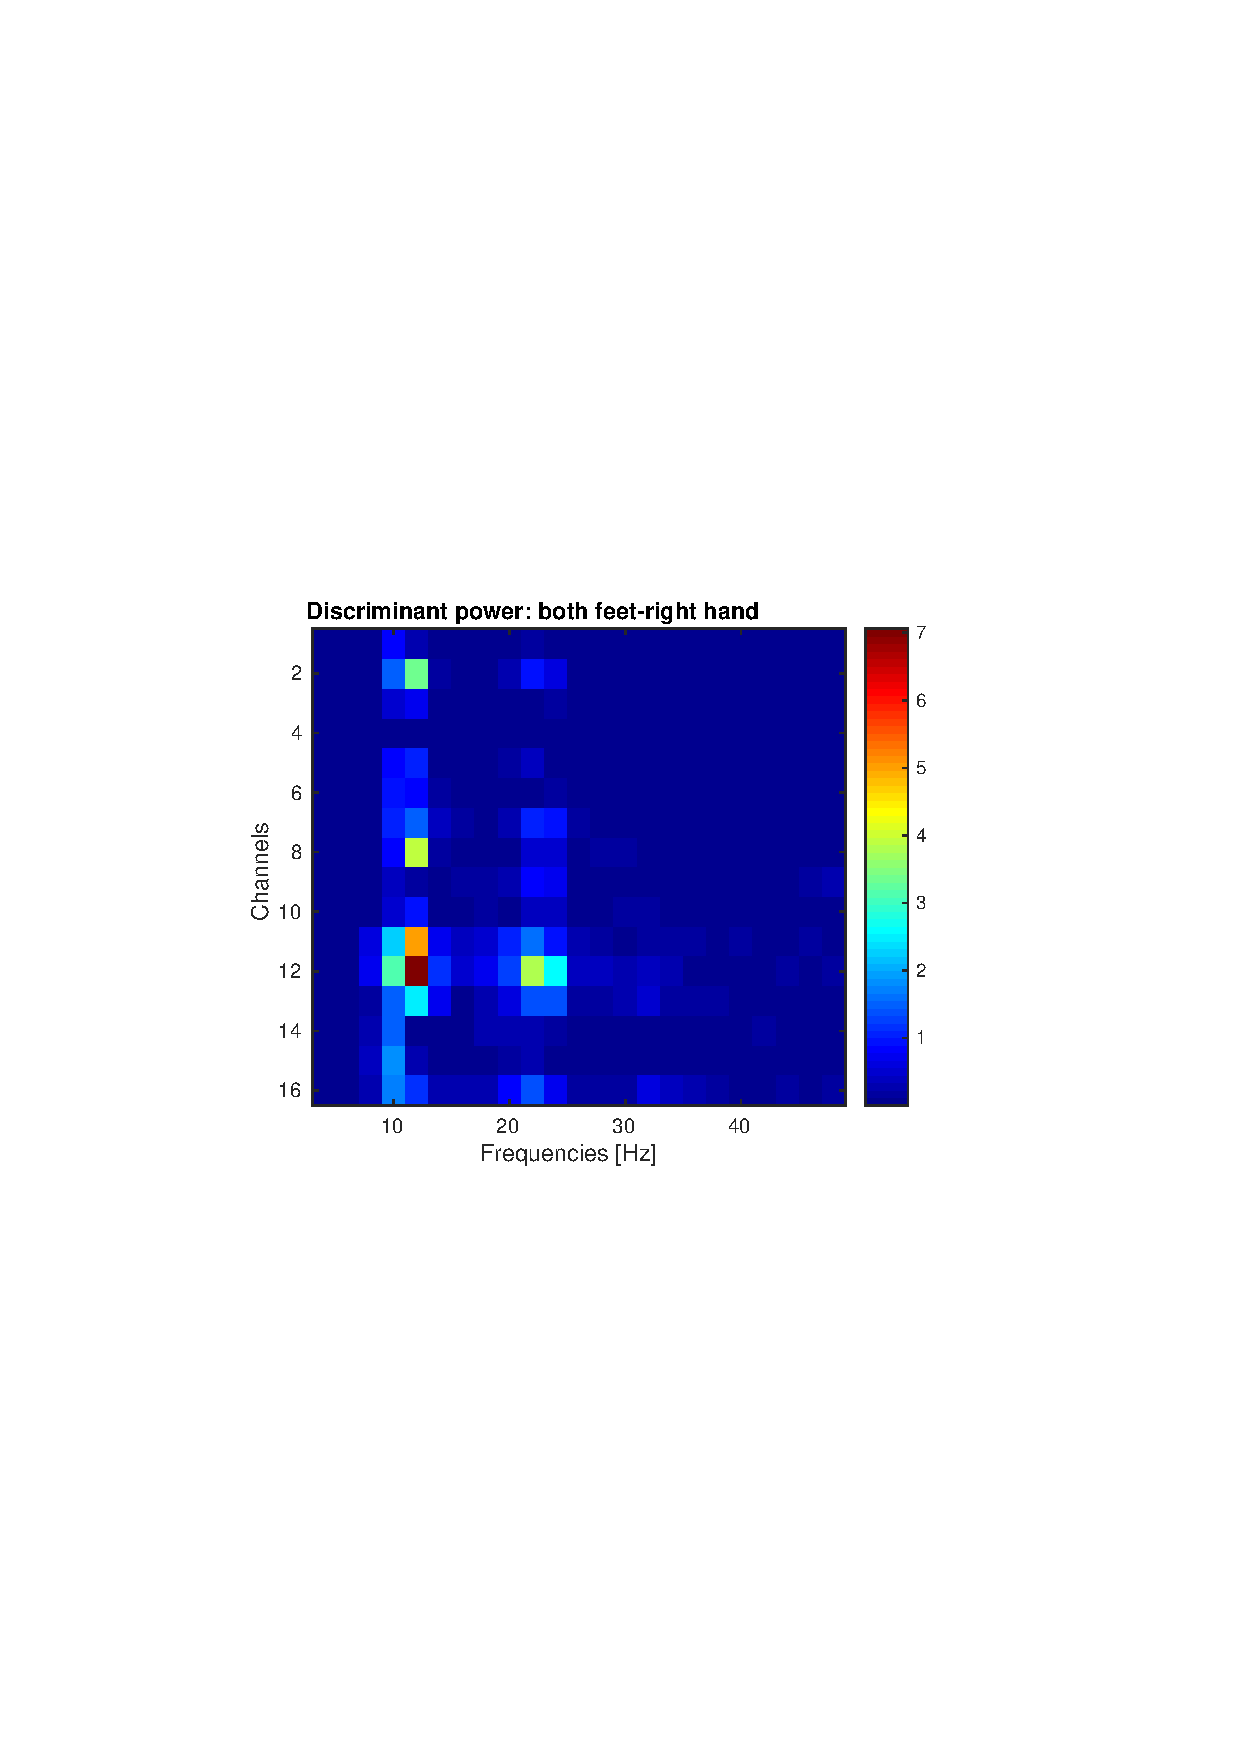
\includegraphics[width = \textwidth]{images/DP_RHBF.pdf}
   \caption{Discriminant power for the different features (channel,frequency) in the discrimination of the classes ``right hand'' and ``both feet''.}
   \label{fig:DP_RHBF}
\end{figure}
\begin{figure}[h!]
   \centering
   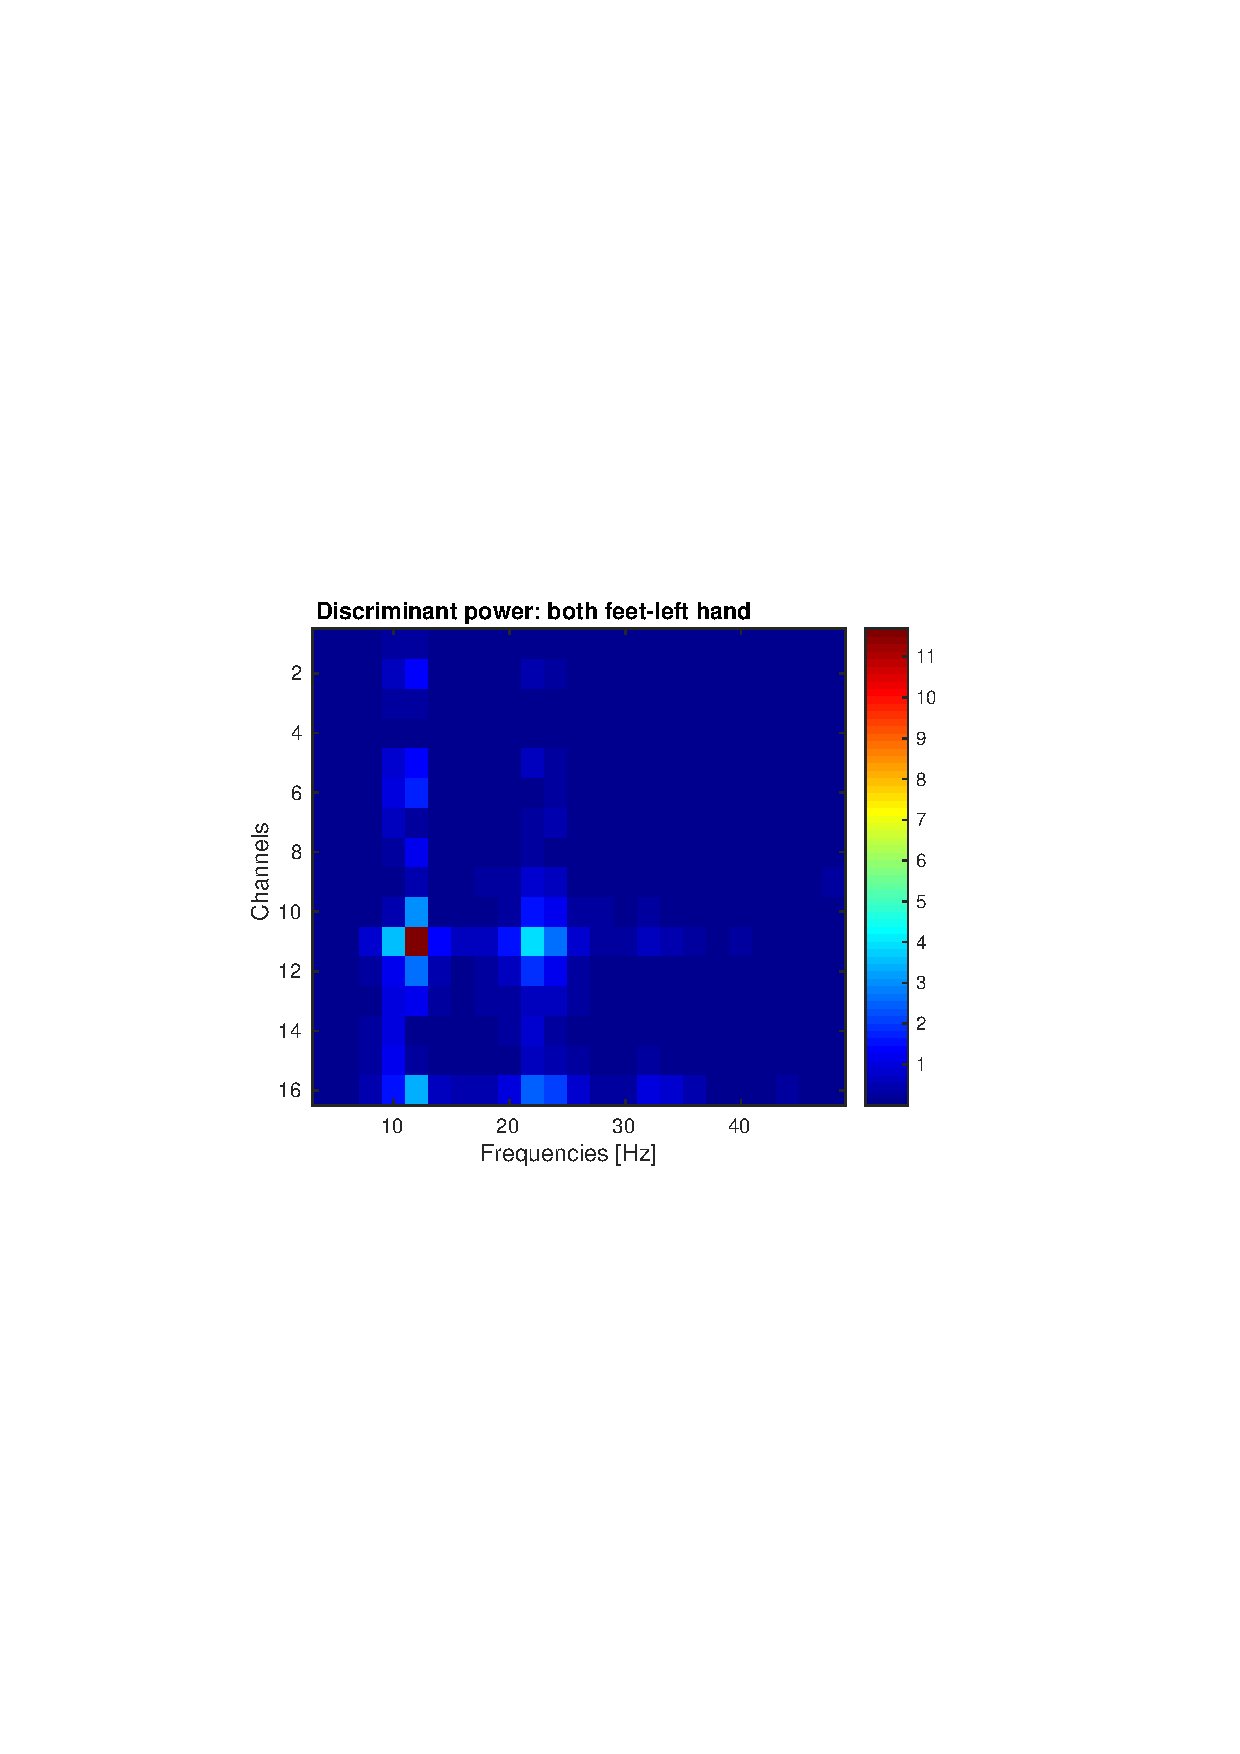
\includegraphics[width = \textwidth]{images/DP_LHBF.pdf}
   \caption{Discriminant power for the different features (channel,frequency) in the discrimination of the classes ``left hand'' and ``both feet''.}
   \label{fig:DP_LHBF}
\end{figure}
The highest discriminant power for the two cases where the ``left hand'' class is involved is in the couple (channel,frequency) = $(11,\unit[12]{Hz})$, in a frequency in the SMR range and in a channel in the right side of the brain.
For the classes \{``right hand'', ``both feet''\}, the highest discriminant power is in the couple $(12,\unit[12]{Hz})$, corresponding to a channel in the left side of the brain.
In this last case, however, the discriminant power is quite lower than in the previous cases.

\subsubsection{Classifier train}
For each couple of classes, the 4 features with the highest discriminant power have been chosen to train the classifier.
The selected features are listed in Table \ref{tab:selFeatures}. \\
\begin{table}
   \centering
   \begin{tabular}{||c c||c c||c c||}
      \hline
      \multicolumn{2}{||c||}{left hand-right hand} & \multicolumn{2}{|c||}{right hand-both feet} & \multicolumn{2}{|c||}{left hand-both feet} \\
      \hline
      (Channel,Frequency)  & DP      & (Channel,Frequency)  & DP     & (Channel,Frequency)  & DP \\
      \hline
      $(11,\unit[12]{Hz})$ & $10.37$ & $(12,\unit[12]{Hz})$ & $7.06$ & $(11,\unit[12]{Hz})$ & $11.68$ \\
      $(11,\unit[24]{Hz})$  & $4.86$  & $(11,\unit[12]{Hz})$ & $4.98$ & $(11,\unit[22]{Hz})$ & $3.90$  \\
      $(10,\unit[12]{Hz})$ & $4.65$  & $(8,\unit[12]{Hz})$  & $3.92$ & $(11,\unit[10]{Hz})$ & $3.58$  \\
      $(11,\unit[22]{Hz})$ & $4.14$  & $(12,\unit[22]{Hz})$ & $3.84$ & $(16,\unit[12]{Hz})$ & $3.30$  \\
      \hline
   \end{tabular}
   \caption{Features selected for classifier train with their discriminant power.}
   \label{tab:selFeatures}
\end{table}
A classifier associates each point in the 4 dimensional space of selected features to its posterior probability of belonging to each class, and associates the point to the class which has the higher posterior probability.
Four different classification techniques are compared in this section, by computing the single sample accuracy for both the test and the train data.
The tested classification techniques are ``linear discriminant analysis'' (\textit{lda}), ``quadratic discriminant analysis'' (\textit{qda}), ``k-nearest neighbor classification'' (\textit{knn}) and ``gaussian classification'' (\textit{gau}).
The results of the classification are listed in Table \ref{tab:class}.
\begin{table}
   \centering
   \begin{tabular}{|c|c|cccc|}
      \hline
      & & lda & qda & knn & gau \\
      \hline
      \multirow{2}{*}{left hand-both feet} & \textbf{Train data} & $91.7\%$ & $94.3\%$ & $94.4\%$ & $91.3\%$ \\
      & \textbf{Test data} & $81.9\%$ & $82.3\%$ & $84.5\%$ & $80.1\%$ \\
      \hline
      \multirow{2}{*}{left hand-right hand} & \textbf{Train data} & $75.6\%$ & $71.8\%$ & $77.0\%$ & $75.2\%$ \\
      & \textbf{Test data} & $73.2\%$ & $70.1\%$ & $73.9\%$ & $72.3\%$ \\
      \hline
      \multirow{2}{*}{right hand-both feet} & \textbf{Train data} & $87.7\%$ & $88.2\%$ & $89.0\%$ & $88.6\%$ \\
      & \textbf{Test data} & $80.1\%$ & $83.8\%$ & $82.2\%$ & $82.6\%$ \\
      \hline
   \end{tabular}
   \caption{Single sample accuracy for the tested classifiers for both train and test data.}
   \label{tab:class}
\end{table}

\section{Online analysis}
The ``online'' analysis uses the classifier calculated in the previous section to assign each trial to its class.
``Online'' data belongs to two different classes, ``left hand'' and ``both feet''.
The data are analyzed by simulating the loop used to control an external device using SMR BCI: they are divided into windows of $\unit[0.5]{s}$ each, separated by $\unit[62.5]{ms}$ each, simulating the buffering of data, and the PSD is computed separately for each window.
The features selected in the ``offline'' analysis are extracted from the PSD and are given as input to the classifier, that outputs the posterior probability for the two classes.
Since posterior probability are often quite uncertain, an evidence accumulation framework is used.
The chosen accumulation framework outputs the probability $P_t(i)$ for the class $i \in \{0,1\}$ at time $t$ as
\begin{equation}
   P_t(i) = \alpha P_{t-1}(i) + (1-\alpha) pp_t(i),
   \label{eq:accum}
\end{equation}
where $pp_t(i)$ is the posterior probability of class $i$ at time $t$ and $\alpha$ is the smoothing parameter.
The initial point is $P_0(i) = pp_0(i)$ for both $i=0$ and $i=1$.
Once $P_t(i) > \theta$, with $\theta$ a chosen threshold, the trial is assigned to class $i$. \\
The accuracy at trial level is computed as the number of trials correctly classified over the total number of trials.
Different values of the smoothing parameters have been tested, all with a threshold $\theta = 0.99$.
The results are listed in Table $\ref{tab:online}$.
\begin{table}
   \centering
   \begin{tabular}{|c|cccc|}
      \hline
      $\alpha$ & lda      & qda      & knn      & gau     \\
      \hline
      $0.01$  & $60.8\%$ & $60.0\%$ & $65.8\%$ & $80.8\%$ \\
      $0.05$  & $60.8\%$ & $61.7\%$ & $66.7\%$ & $83.3\%$ \\
      $0.1$   & $60.8\%$ & $61.7\%$ & $69.1\%$ & $82.5\%$ \\
      $0.2$   & $64.1\%$ & $62.5\%$ & $71.6\%$ & $75.8\%$ \\
      $0.3$   & $64.1\%$ & $62.5\%$ & $75.8\%$ & $71.6\%$ \\
      $0.4$   & $65.0\%$ & $65.0\%$ & $70.8\%$ & $70.8\%$ \\
      \hline
   \end{tabular}
   \caption{Accuracy at trial level for different values of the smoothing parameter.}
   \label{tab:online}
\end{table}
The table shows that, in the range of tested smoothing parameters, the best classifiers are the gaussian and the k-nearest neighbor ones.
The analysis, however, was limited by the fact that the data used in the ``online'' analysis are taken from a real ``online'' session, where the duration of the trial is given by the time the classifier and the accumulation framework used in the session need to discriminate between the classes.
Therefore, the analysis must be restricted to classification techniques giving a result in lower average time than those used in the real ``online'' session. \\
Among the tested classifiers, the one giving the better results is the gaussian classifier with smoothing parameter $\alpha = 0.05$, followed by the k-nearest neighbor with $\alpha = 0.3$. \\
In complex, the accuracy at trial level is lower than the accuracy at the single sample level, even for the test data.
This is probably a problem of the non-optimal classification or accumulation techniques used, since the classifier used in the real ``online'' session gives an accuracy at trial level of $95\%$.

\section{Conclusion}
In this report, the results of the different step of the analysis of the SMR data for BCI have been presented.
The data of the ``offline'' session have been used for both the extraction of the most significant features and the train of different types of classifiers, whose single sample accuracy have been compared.
The best single sample accuracy is given by the k-nearest neighbor classifier, when discriminating between the ``left hand'' and ``both feet'' classes (single sample accuracy of $94.4\%$ for the train data and $84.5\%$ for the test data.
Then the ``online'' loop has been simulated, using the different classifiers calculated using ``offline'' data and an exponential evidence accumulation framework with different values of the smoothing parameter.
The best results have been obtained using the gaussian classifier with smoothing parameter $\alpha = 0.05$, giving an accuracy of $83.3\%$ at trial level.
The much lower accuracy than the one of the real ``online'' session, recovered by looking at the number of HIT and MISS events, suggests that the chosen classification technique is suboptimal and that a better classification or evidence accumulation techniques should be used for BCI.
